
\section{Background}
We present the framework of GANs starting with the original paper by Ian Goodfellow \cite{goodfellow2014generative} then describe more recent advances in a chronological order, as depicted in Figure \ref{fig:background-timeline}. 
% Summarize a few notable approaches/papers tackling the same problem. The selection should cover different possible techniques that can be (have been) used for the same task with success. Also, it is good to mention other recognition/synthesis tasks that use the same deep learning technique as yours. (1-2 pages)

\begin{figure}
\centering
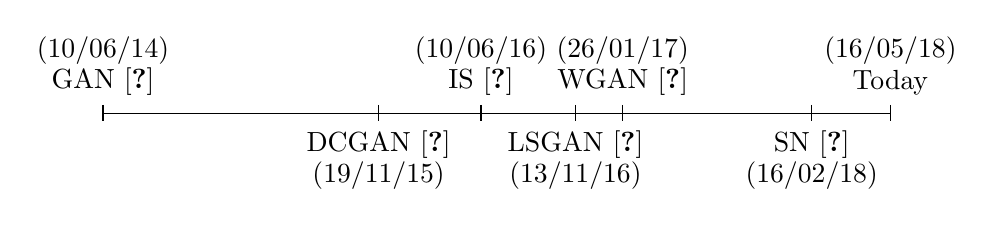
\begin{tikzpicture}
\draw (0,0) -- (10,0);

% draw vertical lines
\foreach \x in {0,3.5,4.8,6.0,6.6,9.0,10.0}
\draw (\x cm,3pt) -- (\x cm,-3pt);

% draw nodes
% 1 yr is roughly 2.5 units
\draw (0,0) node[above=3pt] {GAN \cite{goodfellow2014generative}};
\draw (0,0) node[above=14pt] {(10/06/14)};

\draw (3.5,0) node[below=3pt] {DCGAN \cite{DBLP:journals/corr/RadfordMC15}};
\draw (3.5,0) node[below=14pt] {(19/11/15)};

\draw (4.8,0) node[above=3pt] {IS \cite{salimans2016improved}};
\draw (4.8,0) node[above=14pt] {(10/06/16)};

\draw (6,0) node[below=3pt] {LSGAN \cite{mao2017least}};
\draw (6,0) node[below=14pt] {(13/11/16)};

\draw (6.6,0) node[above=3pt] {WGAN \cite{arjovsky2017wasserstein}};
\draw (6.6,0) node[above=14pt] {(26/01/17)};

\draw (9.0,0) node[below=3pt] {SN \cite{salimans2016improved}};
\draw (9.0,0) node[below=14pt] {(16/02/18)};

\draw (10.0,0) node[above=3pt] {Today};
\draw (10.0,0) node[above=14pt] {(16/05/18)};

\end{tikzpicture}
\caption{Major contributions in the field of Generative Adversarial Networks.}
\label{fig:background-timeline}
\end{figure}


% 2014 jun 10: GAN
% 2015 nov 19: DCGAN
% 2016 jun 10: IS
% 2016 nov 13: LSGAN
% 2017 jan 26: WGAN 
% 2018 feb 16: SN  
% 2018 may 16: Today 

In this work, we consider all of the techniques mentioned in Figure \ref{fig:background-timeline} except LSGAN \footnote{As we progressed in our work, we figured out it was more relevant to investigate further with WGAN-related techniques than implementing a broad spectrum of techniques without really going in-depth.}.

\subsection{Generative Adversarial Networks} 
Generative Adversarial Networks (GANs) were first introduced in \cite{goodfellow2014generative}. They are a class of generative models trained in a adversarial manner by opposing two networks: a generative network $G$ that learns the data distribution and a discriminative network $D$ that tries and estimates the probability that a given sample came from the real training data rather than a generation from $G$. 
 
The objective for $G$ is to maximize the probability of $D$ making a mistake, and the objective for $D$ is to minimize that same probability. This framework corresponds to a minimax two-player game. In the space of arbitrary functions $G$ and $D$, a unique equilibrium solution exists, with $G$ recovering the real data distribution and $D$ equal to 0.5 everywhere, meaning it's unable to distinguish the real images from the ones generated by $G$. Since $G$ and $D$ are (de-)convolutional networks, both can be trained using available backpropagation techniques.

To learn the distribution $p_g$ over the real data $\bm{x}$, $G$ starts from sampling input variables $\bm{z}$ from a distribution of our choice $p_z(\bm{z})$, then maps the input variables $\bm{z}$ to space $G(\bm{z}; \theta_g)$ that should, after training, resemble the training data space. The discriminator, $D$, maps images to a boolean $D(\bm{x}; \theta_d)$ indicating whether images are from training data or generated from $G$. The orignal minimax objective for GANs is defined as:
\begin{equation}
\label{eq_gan}
\min_G \max_D V_{\text{\tiny GAN}}(D, G) = \mathbb{E}_{\bm{x} \sim p_{\text{data}}(\bm{x})}[\log D(\bm{x})] + \mathbb{E}_{\bm{z} \sim p_{\bm{z}}(\bm{z})}[\log (1 - D(G(\bm{z})))] .
\end{equation}

\subsection{Deep Convolutional Generative Adversarial Networks}
Building upon Goodfellow's work \cite{goodfellow2014generative}, Radford et al. apply the GAN framework to computer vision, bridging the gap between the success of Convolutional Neural Networks (CNNs) for supervised learning and GANs for unsupervised learning \cite{DBLP:journals/corr/RadfordMC15}. Training on various image datasets, authors show that the adversarial pair learns a hierarchy of features in both the generator and discriminator. 

\subsection{Inception Score}
The Inception Score (IS) is first presented in \cite{salimans2016improved}. This work (originating from OpenAI, whose team includes author of the original GAN paper Ian Goodfellow) presents a variety of new architectural features and training procedures meant to improve the training of GANs. Amongst other things, authors make the observation that GANs lack an objective function, which making it difficult to compare the performance of different models. In the context of image generation, an intuitive performance metric can be obtained by human annotators assessing the quality of the generated images. However, this method isn't as scalable as one would wish for obvious reasons. The inception score is proposed as an alternative, and is shown to correlate well with human evaluation. 

We describe the method briefly. By applying the Inception model \cite{inceptionv2} to all generated images, we get the conditional label distribution $p(y|\bm{x})$. Images that contain meaningful objects should have a conditional label distribution $p(y|\bm{x})$ with low entropy. Moreover, we expect the model to generate varied images, so the marginal $\int p(y|\bm{x} = G(z))dz$ should have high entropy. By combining these two requirements, the proposed metric becomes: 

%$\exp( \mathbb{E}_{\bm{x}} \text{KL} (p(y|\bm{x})||p(y)))$, where results are exponentiated so that values are easier to compare.
% In \cite{Barrat2018IS} the Inception score is defined  as:
\begin{equation}
\label{eq_IS}
\begin{split}
\text{IS}(G) = \exp \big(\mathbb{E}_{\bm{x} \sim p_{\text{data}}(\bm{x})}D_\text{KL}(p(y|\bm{x})||p(y))\big).
\end{split}
\end{equation}

Here $D_{KL}$ is known as the Kullback-Leibler divergence and it measures how one probability distribution diverges from another by using a logarithmic difference:
\begin{eqnarray}
	D_{\mathrm {KL} }(P\|Q)=\int _{-\infty }^{\infty }p(x)\,\log {\frac {p(x)}{q(x)}}\,dx,
\end{eqnarray}
where $p(y|\bm{x})$ is the conditional label distribution while $p(y)$ is the  marginalized label distribution, i.e. $p(y)=\int_{\bm{x}} (p(y|\bm{x})p_g(\bm{x}) d\bm{x}$. In order to calculate the score we replace $p(y)$ with the empirical marginal class distribution $\hat{p}(y) = \sum^N_{i=1} p(y|\bm{x}^i)$ and estimate the expectation using the basic Monte Carlo estimator yielding:

\begin{equation}
\label{eq_IS2}
\begin{split}
\text{IS}(G) = \exp\left(\sum^N_{i=1}D_{\mathrm{KL}}(p(y|\bm{x}^i)||\hat{p}(y))\right).
\end{split}
\end{equation}


\subsection{WGAN}
The Wasserstein GAN (WGAN) algorithm is proposed as a consequence to various  observations on how we usually measure the distance between the model distribution and the real distribution. In fact, the choice of divergence functions has a huge impact on how the discriminator will manage to classify samples as real or fake, and in turn how the generator will be led to adjust its parameters to mimic the real distribution. Authors show how the Earth Mover (EM) distance behaves in comparison to popular probability distances and divergences used in the context of learning distributions. WGANs are introduced by making GANs minimize a reasonable and efficient approximation of the EM distance, working under the assumption that the discriminator functions are $K$-Lipschitz continuous. For a parameterized family of functions $\{ f_w \}_{w \in \mathcal{W}}$ that all have the $K$-Lipschitz continuity property, the discriminator objective is defined as:
\begin{equation} \label{eq:wgan}
\max_{w \in \mathcal{W}} \mathbb{E}_{x \sim p(x)}[f_w(x)] -
\mathbb{E}_{z \sim p(z)} [f_w(g_\theta (z)].
\end{equation}
As a result, one of the most compelling practical benefits of WGANs is the ability to continuously estimate the EM distance by training the discriminator to optimality. Various ways to ensure Lipschitz continuity are described, including gradient penalty or weight clipping. For the latter, however, author note that it is ``clearly terrible way to enforce a Lipschitz constraint''.
% Recommended clip limit is 0.01

\subsection{Spectral Normalization}
\label{sec:bg-sn}

Spectral normalization \cite{miyato2018spectral} was introduced in an effort to try and make the training of GANs more stable and the original paper received very positive criticism. \footnote{As a matter of fact, this has been posted on the peer-reviewing platform \url{https://openreview.net/forum?id=B1QRgziT-}:
\begin{quote}
\textit{``This is a great paper! I don't think this paper explains the importance of its results nearly enough and I'm concerned that it may not be obvious what a breakthrough it is just from skimming the abstract.''} - Ian Goodfellow
\end{quote}
}. As we noted in the previous section, Lipschitz continuity is a property of interest for GANs. More specifically, the assumption for the loss of Wasserstein GANs is that the functions yielded by the discriminator are $K$-Lipschitz continuous for some constant $K$. Spectral normalization aims to control the Lipschitz constant of this discriminator function $f$ by constraining the spectral norm of each layer 
$
g_l : \bm{h}_{l-1} \mapsto W^{l} \bm{h}_{l-1}
$. We briefly review the method, but the interested reader will find a more comprehensive explanation in the original paper. 

By definition, the Lipschitz norm $\|g\|_{\rm Lip}$ is equal to $\sup_{\bm{h}} \sigma (\nabla g(\bm{h}))$, with $\sigma (A)$ being the spectral norm of the matrix $A$ (which is equivalent to the largest singular value of $A$). Therefore, for a linear layer $g_l$, the norm is given by $\|g_l\|_{\rm Lip} = \sup_{\bm{h}} \sigma (\nabla g_l(\bm{h})) = \sup_{\bm{h}} \sigma (W_l) = \sigma (W_l) $. Now, if the Lipschitz norm of the activation function $\|a_l\|_{\rm Lip}$ is equal to 1 (a condition that ReLU or Leaky ReLU satisfy \todo{cite}), we can use the composition inequality $\|g_1\circ g_2\|_{\rm Lip}\leq\|g_1\|_{\rm Lip}\cdot\|g_2\|_{\rm Lip}$ and define the bound on $\|f\|_{\rm Lip}$:
%
% The last layer should not have an activation function in this context
% However we can omit (nobody will notice I guess) or add an indicator function as exponent
%
\begin{align}
 	\|f\|_{\rm Lip} \leq &  \prod_{l=1}^{L+1} \|a_{l}\|_{\rm Lip} \|g_{l}\|_{\rm Lip} = \prod_{l=1}^{L+1} \sigma (W^{l}). \label{eq:ineq_lip}
\end{align}
For each layer, spectral normalization alters the weight matrix $W_l$ so that it satisfies the Lipschitz constraint $\sigma (W_l) = 1$:
\begin{align}
\bar{W_l}_{\rm SN}(W_l) := W_l / \sigma (W_l) \label{eq:sn},
\end{align}
enforcing the upper bound of 1 for $\|f\|_{\rm Lip}$ using the inequation \ref{eq:ineq_lip}.
